\documentclass[a4]{seminar}
%%% ESTAH EM LATIM .....
\usepackage[utf8x]{inputenc}
\usepackage[portuges,brazil]{babel}
\usepackage{fancybox}
%\usepackage{fancyhdr}
\usepackage[normalem]{ulem}
%%%%\newcommand{\ro}{${}^{\underline{\circ}}$\ }
%%%http://www.artofproblemsolving.com/LaTeX/AoPS_L_GuideLay.php
\usepackage{float,epsfig}

\newcommand{\bd}{\begin{description}}
\newcommand{\ed}{\end{description}}

%%% com {slide*} {\ldots}  vai para portrait 
\newcommand{\bs}{\begin{slide}}
\newcommand{\es}{\end{slide}}

\newcommand{\bv}{\begin{verbatim}}
\newcommand{\ev}{\end{verbatim}}

%\newcommand{\prefixo_1}{{\footnotesize \begin{tabular}{l||r} \begin{minipage}[t]{0.45\textwidth}}

%%%%%%%configura tamanho slides%%%%%%%%%%%%%%%%%%
\setlength{\pdfhorigin}{1truein}
\setlength{\pdfvorigin}{1truein}
\makeatletter
\setlength{\pdfpagewidth}{\strip@pt\paperheight truept}
\setlength{\pdfpageheight}{\strip@pt\paperwidth truept}
\makeatother
%%%%%%%%%%%%%%%%%%%%%%%%%%%%%%%%%%%%%%%%%%%%%%%%%%
\slideframe{Oval} %% vem do fancy box...
%%Oval}\shadowbox \doublebox {texto aqui....}
\newcommand{\heading}[1]
 {
  \begin{center}
    \large\bf
    \shadowbox{#1}
  \end{center}
  \vspace{1ex minus 1ex}
}

%\usepackage[dvips]{graphicx}
%%\usepackage{float} não funcionam
%\fancyfoot[C]{\thepage}
%\fancyhead[RE,RO]{\thepage}
%\fancyhead[LE,LO]{{\small COCA}}

\usepackage{amsmath}
\usepackage{amsfonts}
\usepackage{amssymb}

%%\portraitonly
\topmargin        -1.0cm   
\paperheight      297mm
\paperwidth       210mm

\slideheight      15cm
\slidewidth       23cm

\ptsize{8}
%\setcounter{page}{0}
%\setcounter{page}{16}

%\slidereset{\setcounter{page}{16}}
\restylefloat{figure}   %%%% obrigatório... pelo [H]
%%\linespread{1.9}
\begin{document}
\bs
\begin{center}

\begin{large}Tutorial: \\
\underline{Brincando com \LaTeX}\footnote{A proposta
desse tutorial
é deixar o leitor pronto para fazer seus textos em
\LaTeX . Logo,
alguns detalhes são omitidos propositalmente. Ou seja,  este  tutorial é um  
``{\em ready-to-run}" \/ do \LaTeX . }\\
\end{large}
\vskip 1cm
Claudio Cesar de Sá \\
Charles Christian Miers \\
Rogério Eduardo da Silva\\
\vskip 1cm
{\small
Grupo Colméia  (http://www.colmeia.udesc.br/)\\
Departamento de Ciência da Computação -  DCC \\
Centro de Ciências Tecnológicas - CCT \\
Universidade do Estado de Santa Catarina - UDESC\\
}
%%\vskip 2cm
\vfill
\end{center}
\es

\bs
\heading{O que é o \LaTeX \/?}
\begin{description}
\item[$\checkmark$]   O \LaTeX \/ é um
processador de texto, de código aberto,
portável, e padrão para comunidade
científica;
\item[$\checkmark$] Como processador de texto, o mesmo
  {\bf é orientado a conteúdo}, e não às formas e 
estéticas do texto;
   
\item[$\checkmark$] O detalhe do ``{\em WYSIWYG}''
(``{\em what you see is what you get}'') é uma
consequência do ato do texto ser processado;

\item[$\checkmark$] Tudo no \LaTeX \/ é fortemente
documentado em livros, e com um rico (e muito) material na WEB 
(procure por: ``{\em \LaTeX \/ Tutorial, Guide, Examples, Tips, ...) }";

\item[$\checkmark$] http://www.artofproblemsolving.com/LaTeX/AoPS\_L\_GuideLay.php
\item[$\checkmark$] ``{\em \LaTeX \ does not support drawing figures in WYSIWYG way}";
\item[$\checkmark$] Bem, o \LaTeX \/ não é tudo, mas é
100\%!
 \end{description}

\es


\bs

\heading{Requisitos e Instalação}

\begin{description}
\item[$\checkmark$] Um editor ordinário (aquele que
  estiveres acostumado), padrão ASCII (Bloco de Notas por exemplo).
  Evite WordŽs e similares que tem formatação interna; 
 \item[$\checkmark$] Um dos muitos compiladores \LaTeX
 \/   existentes, gratuito, e disponíveis em
  vários sites na WEB. Aconselha-se o MiKTeX (www.miktex.de).
\end{description}


\heading{Procedimento Básico}

\begin{enumerate}
  \item Edite o texto desejado, sob a
  formatação \LaTeX, em um editor ASCII
  qualquer;

  \item Compile este texto com o comando:\\
  {\mbox latex  nome\_do\_arquivo.tex};

\item Se houver erros, retorne ao passo 1;

\item Confira a saída no
    arquivo: nome\_do\_arquivo.dvi. A extensão
    ``{\em dvi}", significa: ``{\em Device
    Independent}". Para visualizar este
    arquivo use programas: {\bf xdvi} no Linux
    ou {\bf yap} (``{\em Yet Another
    Previewer}") no Windows;

  \item Se quiser imprimir a partir do formato ``{\em
  \*.dvi}", este já está pronto para impressora;

  \item Se quiser converter para o formato
  Postscript (\*.ps), use o comando: \\
  {\mbox dvips -o arq\_saida\_em\_ps.ps
  nome\_do\_arquivo.dvi};

\item Se quiser converter diretamente para
    PDF (``{\em Portable Document Format}"),
    repita o passo 2, com:\\ {\mbox pdftex
  nome\_do\_arquivo.tex} \\
  O arquivo de saída   será {\mbox pdftex
  nome\_do\_arquivo.pdf},  pronto para ser
  lido no Acrobat Reader, disponível em
  qualquer lugar.
\end{enumerate}

Algumas variações sobre os dois últimos passos. Fica a
critério do que o
usuário mais se adaptar.

\es
%%%%%%%%%%%%%%%%%%%%
\bs
\heading{Resumindo estes Passos}
\begin{figure}[H]
\begin{center}
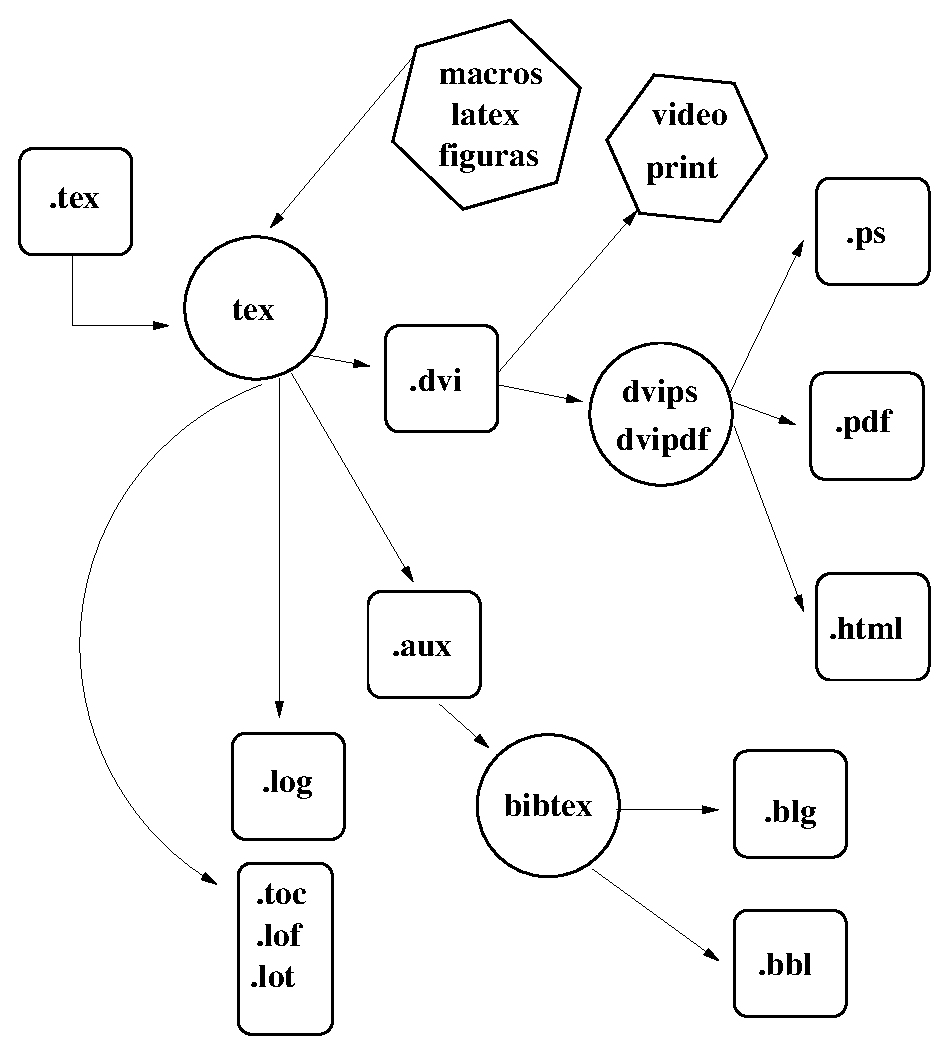
\includegraphics[height=6cm,width=9cm]{figuras/passos_compila.eps}
\caption{Principais Passos}
\label{xx}
\end{center}
\end{figure}
\es
%%%%%%%%%%%%%%%%%%%%%%%%%%%%%%%%%%%%%%%%%%%%%
\bs
\heading{Montando um Documento \LaTeX}
{\small  %%% para as letras nao ficarem muito grandes
\begin{tabular}{l||r}
\begin{minipage}[t]{0.45\textwidth}

\fbox{ \parbox [c]{0.92\textwidth}{
$\backslash$documentclass[oções]\{estilo\} \\ 
  \fbox{ \parbox [c]{0.85\textwidth}{ 
\begin{center}  
 Uma área de preâmbulo. Local onde se inicia
 com as
definições do documento.
\end{center}
}} 
$\backslash$begin\{document\}
\fbox{\parbox [c]{0.85\textwidth}{ 
\begin{center}  O corpo  do documento propriamente
dito. Podendo se incluir arquivos, como outros
textos, figuras, etc, em tempo de compilação.
\end{center}
}}
\fbox{\parbox [c]{0.85\textwidth}{ 
\begin{center} 
Alguns comandos para finalização.
Exemplo: gerar automáticamente 
referências bibliográficas, 
índices remissivos, etc.
\end{center}
}}
$\backslash$end\{document\}
}}

\end{minipage}

&  %%% final do tabular mais externo....

\begin{minipage}[t]{0.45\textwidth} 
\begin{verbatim}


\end{verbatim}
\end{minipage}
\end{tabular}
}

\es
%%%%%%%%%%%%%%%%%%%%%%%%%%%%%%%%%%%%%%%%%%%%%%%%%%%%%%%%%%%

\bs
\heading{Construindo um Arquivo \LaTeX}
%%\vfill

{\footnotesize
\begin{tabular}{l||r}
\begin{minipage}[t]{0.45\textwidth}

\begin{center}
{\Large {\bf Assim Caminha a \ldots}}\\
Por Claudio e outros.
\end{center}

\section{Introdução}
Era uma vez, ......
\section{Conclusão}
\ldots \ldots \ldots \ldots \ldots \\
Mas, com o passar dos anos, nos acostumamos
as diabruras do \LaTeX \/. Toda história
tem um final feliz!

\end{minipage}
& %%% final do tabular mais externo....

\begin{minipage}[t]{0.45\textwidth} 
\begin{verbatim}
\documentclass[12pt]{article}
\usepackage[portuges,brazil]{babel}

\begin{document}
\begin{center}
{\Large {\bf Assim Caminha a \ldots}}\\
Por Claudio e outros.
\end{center}

\section{Introdução}
Era uma vez, ......
\section{Conclusão}
\ldots \ldots \ldots \ldots \ldots \\
Mas, com o passar dos anos, nos acostumamos
as diabruras do \LaTeX \/. Toda história
tem um final feliz!
\end{document}

\end{verbatim}
\end{minipage}
\end{tabular}
}
\es



%%%%%%%%%%%%%%%%%%%%%%%%%%%%%%%%%

\bs
\heading{Ampliando a Idéia}
%%\vfill

{\footnotesize
\begin{tabular}{l||r}
\begin{minipage}[t]{0.45\textwidth}

\section{Evolução do \LaTeX }
Era uma vez ......
\subsection{Organizando o Texto}
As sub-seções são interessantes
\subsubsection{Mais Uma Sub-seção}
E esta  também \ldots
\subsubsection{Neste Mesmo Nível}
E esta  também \ldots
\subsubsection{Finalmente \ldots}
Legal, temos uma numeração automática,
de seções, sub-seções, e assim sucessivamente!

\end{minipage}
& %%% final do tabular mais externo....

\begin{minipage}[t]{0.45\textwidth} 
\begin{verbatim}
\section{Evolução do \LaTeX }
Era uma vez ......
\subsection{Organizando o Texto}
As sub-seções são interessantes
\subsubsection{Mais Uma Sub-seção}
E esta  também \ldots
\subsubsection{Neste Mesmo Nível}
E esta  também \ldots
\subsubsection{Finalmente \ldots}
Legal, temos uma numeração automática,
de seções, sub-seções, e assim sucessivamente!
\end{verbatim}
\vskip 0.5cm
\fbox{\fbox{\parbox [c]{5cm}{ \begin{center} {\Large \uwave{ O texto segue se organizando lentamente!}}\end{center}}
}}
%%\framebox[0.45\textwidth][c]{O texto segue se organizando lentamente}
%%\fbox{\fbox{!}}
\end{minipage}
\end{tabular}
}
\es

%%%%%%%%%%%%%%%%%%%%%%%%%%%%%%%%%

\bs
\heading{Os Tamanhos de Letras}
%%\vfill
{\small
%footnotesize
\begin{tabular}{l||r}
\begin{minipage}[t]{0.45\textwidth}
{\tiny a menor } ou {\scriptsize ainda esta } \\
{\footnotesize aumentado}, {\small muito usada}\\
{\large aumentando},  {\Large subindo},\\
{\LARGE e mais}, {\huge quase lá}, \\
{\Huge já  é o suficiente !} \\
\vskip 0.5pt
Opcionalmente: \\
\begin{footnotesize}
\begin{center}
Tudo em em \\
blocos, por palavra, ou \\
com quebra de linha!
\end{center}
\end{footnotesize}

\end{minipage}
& %%% final do tabular mais externo....
\begin{minipage}[t]{0.45\textwidth} 
\begin{verbatim}
{\tiny a menor } ou
{\scriptsize ainda esta } \\
{\footnotesize aumentado}, 
{\small muito usada}\\
{\large aumentando},  {\Large subindo},\\
{\LARGE e mais}, {\huge quase lá}, \\
{\Huge já  é o suficiente !} \
\vskip 0.5pt
Opcionalmente: \\
\begin{footnotesize}
\begin{center}
Tudo em em \\
blocos, por palavra, ou \\
com quebra de linha!
\end{center}
\end{footnotesize}

\end{verbatim}
\end{minipage}
\end{tabular}
}
\vfill
\begin{center}
\fbox{\fbox{Tudo isto está dentro de um $\setminus$small !}}
\end{center}
\es

%%%%%%%%%%%%%%%%%%%%%%%%%%%%%%%%%%%%%%%%%%%%%%%%%%%%%%%%%%%%%%%%%%

\bs
\heading{Os Estilos  das Letras}
%%\vfill
{\normalsize
\begin{tabular}{l||r}
\begin{minipage}[t]{0.45\textwidth}
{\rm romano },  {\em enfatizado } ,\\
{\bf negrito}, {\it  itálico},  ``{\sl slantado}",\\
``{\sf sherifado}",  {\sc maiúsculo}, {\tt máquina de escrever}.\\

Opcionalmente: \\
\begin{center}
{\em  
Tudo em em \\
blocos, por palavra, ou \\
ainda com quebra de linha!
}

\vskip 0.7cm
\underline{Carácteres Especiais:} \\
\textbf{\$ \ \& \ \% \ \# \ 
\{ \ \} \  \_  \ $\backslash $ } 

\end{center}

\end{minipage}
& %%% final do tabular mais externo....
\begin{minipage}[t]{0.45\textwidth} 
\begin{scriptsize}
\begin{verbatim}
{\rm romano },  {\em enfatizado } ,\\
{\bf negrito}, {\it  itálico},  
``{\sl slantado}",\\``{\sf sherifado}",  
{\sc maiúsculo}, {\tt máquina de escrever}.\\

Opcionalmente: \\
\begin{center}
{\em  
Tudo em em \\
blocos, por palavra, ou \\
ainda com quebra de linha!
}

\vskip 0.7cm
\underline{Carácteres Especiais:} \\
\textbf{\$ \ \& \ \% \ \# \ 
\{ \ \} \  \_  \ $\backslash $ } 

\end{center}
\end{verbatim}
\end{scriptsize}
\end{minipage}
\end{tabular}
}
\es
%%%%%%%%%%%%%%%%%%%%%%%

\bs
\heading{Listas}
{\small
%footnotesize
\begin{tabular}{l||r}
\begin{minipage}[t]{0.45\textwidth}
\begin{itemize}
\item Itemized lists are handy.
\item However, don't forget
  \begin{enumerate}
  \item The `item' command.
  \item The `end' command.
  \end{enumerate}
\end{itemize}



\begin{description}
  \item[gnat] A small animal that causes no end of trouble.
  \item[gnu] A large animal that causes no end of trouble.
  \item[armadillo] A medium-sized animal.
\end{description}



\end{minipage}
& %%% final do tabular mais externo....
\begin{minipage}[t]{0.45\textwidth} 


\end{minipage}
\end{tabular}
}

\es

%%%%%%%%%%%%%%%%%%%%%%%%%%%%%%%%%%%%%%%%%%%%%%%%%%%%%%%%%%%%%%%%%%


\bs
\heading{Modo Matemático}

%footnotesize
\begin{tabular}{l||r}
{\small
\begin{minipage}[t]{0.45\textwidth}
\begin{description}

\item[$\checkmark $] Basicamente há dois modos de um texto:
normal e {\em matemático}. Contudo, o matemático
é para fórmulas, equações referenciadas, etc;


\item[$\checkmark $] Adicionalmente, há algumas dezenas
 de símbolos
matemáticos prontos para serem utilizados, mediante
o carregamento do pacotes matemáticos:\\
$\setminus $usepackage\{amsmath\}\\
$\setminus $usepackage\{amsfonts\}\\
$\setminus $usepackage\{amssymb\}\\
Novamente, há necessidade de se ter uma apostila
completa de \LaTeX \ para conhecer todos os símbolos disponíveis;

\item[$\checkmark $] O \LaTeX \  exibe
três modos de se construir fórmulas matemáticas:
\end{description}

\end{minipage}
}
& %%% final do tabular mais externo....

{\footnotesize
\begin{minipage}[t]{0.45\textwidth} 
\begin{enumerate}
\item \underline{Modo simples}: algo como $y(x)=\Sigma^{100}_{n=1}x_n$, onde
esta fórmula foi escrita entre os símbolos {\bf \$ ... \$},
ou {\bf $\setminus $(  ... $\setminus $)} ou ainda: 
{\bf $\setminus $begin\{math\} ... $\setminus $end\{math\}} ;
\item \underline{Modo centralizado}: a fórmula numa
nova linha, centralizada, tal como:
$$
y(x)=\Sigma^{100}_{n=1}x_n
$$
onde a fórmula foi definida entre os símbolos: 
{\bf \$\$ ... \$\$},
ou {\bf $\setminus $[  ... $\setminus $]} ou ainda: 
{\bf $\setminus $begin\{displaymath\} ... $\setminus $end\{displaymath\}} ;

\item \underline{Modo equação}: o qual permite fazer fórmulas com
referências no texto. O ambiente é definido por:
{\bf $\setminus $begin\{equation\} ... $\setminus $end\{equation\}},
\begin{equation}
y(x)=\Sigma^{100}_{n=1}x_n
\label{soma_exemplo}
\end{equation} 

\end{enumerate}
\end{minipage}
}
\end{tabular}

\es



%%%%%%%%%%%%%%%%%%%%%%%%%%%%%%%%%%%%%%%%%%%%%%%%%%%%%%%%%%%%%%%%%%

\bs
\heading{Exemplos Matemáticos}
{\normalsize
%footnotesize
\begin{tabular}{l||r}
\begin{minipage}[t]{0.45\textwidth}

E a fórmula de Eisntein é: $ E = m.c^2 $ \\
$y=\int^{100}_{-99} x^2 dx $ \\
$ \mbox{Xís}= \{ x^{i+j+k}_{k-(j-i)} \mid i,\ j,\ k \ge 9 \}$ \\
$x\succ y \vdash y \sim x $ \vskip 10pt
$x\circledast y \boxtimes z$, $\overrightarrow{abc}$, $\underbrace{abc}$ \vskip 8pt
Numa linha: $y = \frac{a}{b}$ ou  $z=\dfrac{x}{y}$ (AMS)\vskip 8pt

As letras gregas prontas:\\
$\alpha$, $\gamma$, $\Gamma$, $\delta$, $\Delta$, $\zeta$,
$\eta$, $\omega$, $\vartheta$, $\rho$, $\mu^{\lambda+\beta}$,...

Alguns símbolos:\\
\dag, \ddag, \S, \pounds, \copyright, $\sharp$, $\clubsuit$, ...\\
Finalmente, tudo com marcas especiais: $\acute{\mu}$, $\hat{\delta}$, $\vec{\epsilon}$, $\tilde{8}$, $\ddot{o}$, ...

\end{minipage}
& %%% final do tabular mais externo....
\begin{minipage}[t]{0.45\textwidth} 
\begin{verbatim}
$ E = m.c^2 $
\end{verbatim} 

\end{minipage}
\end{tabular}
}


\es





%%%%%%%%%%%%%%%%%%%%%%%%%%%%%%%%%%%%%%%%%%%%%%%%%%%%%%%%%%%%%%%%%%

\bs
\heading{Equações Matemáticas}
\begin{center}
{\small
Sofisticando o uso das expressões matemáticas, e referências
no texto adequadamente, etc.
}
\end{center}
{\small
\begin{tabular}{l||r}
\begin{minipage}[t]{0.45\textwidth}
$$
\dfrac{\pi^2}{6}= \dfrac{1}{1^2}+\dfrac{1}{2^2}+\dfrac{1}{3^2}+\dfrac{1}{4^2} ...
$$
\vskip 0.5cm
\begin{equation}
e^{\pi i} + 1 = 0
\label{eq_euler}
\end{equation}
\begin{center}
Equação de Euler
\end{center} 

Fazendo referência a equação \ref{eq_euler}, 
tem-se ...\\ mas temos de compilar o texto duas 
vezes para a referência \ref{eq_euler} aparecer  
corretamente no texto.

Onde $i$ e $\pi$ em \ref{eq_euler} é definido por:\\
$$
\begin{array}{|l|}
\hline 
i = \sqrt{-1}  \mbox{ \hskip 1cm  e}\\
\pi = 3.1415 ... \\
\hline
\end{array}
$$


\end{minipage}
& %%% final do tabular mais externo....

\begin{minipage}[t]{0.45\textwidth} 
%\begin{flushright}
\begin{verbatim}

\end{verbatim}
%\end{flushright}
\end{minipage}
\end{tabular}
}


\es

\bs
\heading{Tabelas}

{\small
\begin{tabular}{l||r}
\begin{minipage}[t]{0.45\textwidth}
%%Há várias maneiras de se montar tabelas em \LaTeX \ e referenciá-las.
Basicamente tem-se: \textit{tabbing}, \textit{tabular}, \textit{array} (este último, é
 matemático e tem variações).
Usando o {\em tabbing}:\\

\begin{tabbing}
Núm. \=  Nome     \=    {\hskip 1cm} Idade \\
1 \>     Klaus Souza \> {\hskip 1cm} 22 \\
2 \>     Karla Silva \> {\hskip 1cm} 23 \\
... \> ... \> ...
\end{tabbing} 

Usando o {\em tabular}:
\begin{table}[H]
\caption{ Exemplo 2 (acima)}
\label{tab_1}
\begin{tabular}{|c|c|c|} \hline
Usando & o & \textbf{tabular} \\ \hline
Sou  & mais & flexível, \\
tolerante, & e bondoso & que \\
meu & irmão & acima! \\ \hline
\end{tabular} 
\end{table} 

O modo e uso  da tabela \ref{tab_1} é 
fortemente recomendável!
\end{minipage}
& %%% final do tabular mais externo....

\begin{minipage}[t]{0.45\textwidth} 
%\begin{flushright}
\begin{verbatim}

\end{verbatim}
%\end{flushright}
\end{minipage}
\end{tabular}
}

\es



%%%%%%%%%%%%%%%%%%%%%%%%%%%%%%%%%%%%%%%%%%%%%%%%%%%%%%%%%%%%%%%%%%

\bs
\heading{Figuras}
{\small
\begin{tabular}{l||r}
\begin{minipage}[t]{0.45\textwidth}
 \begin{description}
\item [$\divideontimes$]Há vários modos, tipos de figuras,
que podem ser inseridas no texto;
\item [$\divideontimes$] Mais simples e flexíveis, é o
``{\em Encapsulated Postscript}", (.eps);
\item [$\divideontimes$] Adicionar os pacotes:  $\setminus$usepackage\{graphicx\}, $\setminus$usepackage\{float,epsfig\} no preâmbulo do documento;
 \end{description}
    
Exemplificando o básico:
      \begin{figure}[H]
      \centering
      
\includegraphics[width=2cm,height=2cm]{figuras/casa_1.eps}
      \caption{O rótulo desta figura}
      \label{figura_1}
      \end{figure}

E da figura \ref{figura_1} temos uma casa.


 
\end{minipage}

& %%% final do tabular mais externo....

\begin{minipage}[t]{0.45\textwidth} 
%\begin{flushright}
\begin{verbatim}

\end{verbatim}
%\end{flushright}
\end{minipage}
\end{tabular}
}


\es
%%%%%%%%%%%%%%%%%%%%%%%%%%%%%%%%%%%%%%%%%
\bs
\heading{Mais Figuras}
{\small
\begin{tabular}{l||r}
\begin{minipage}[t]{0.45\textwidth}
\begin{center}

\framebox[3cm]{
\begin{figure}[H]

\includegraphics[angle=45,width=2cm,height=2cm]{figuras/dog.jpeg}
\caption{Um animal e seu computador}
\label{figura_2}
\end{figure}
}
\end{center}

Das figuras \ref{figura_1}, \ref{figura_2}, e \ref{figura_3} concluimos
a facilidade de figuras em \LaTeX !

\begin{center}

\framebox[4cm]{
\begin{figure}[H]

\includegraphics[angle=0,width=3.5cm,height=2.5cm]{figuras/casa_2.eps}
\caption{Um animal e seu computador}
\label{figura_3}
\end{figure}
}
\end{center}
Usar o $\setminus$restylefloat\{figure\} no preâmbulo!  
\end{minipage}

& %%% final do tabular mais externo....

\begin{minipage}[t]{0.45\textwidth} 
%\begin{flushright}
\begin{verbatim}

\end{verbatim}
%\end{flushright}
\end{minipage}
\end{tabular}
}


\es


%%%%%%%%%%%%%%%%%%%%%%%%%%%%%%%%%%%%%%%%%%%%%%%%%%%%%%%%%%%%%%%%%%
\bs
\heading{Referências Bibliográficas}
{\small
\begin{tabular}{l||r}
\begin{minipage}[t]{0.45\textwidth}
 Aconselhamos o uso do \underline{\textbf{bibtex}}. Os passos:
\begin{description}
\item [1.] Ter o arquivo em separado de referências no padrão bibtex (consultar manuais
de quais os conteúdos, e como se constrói todos os detalhes. Há programas
prontos que fazem isto automaticamente. Sugestão: faça tudo manualmente 
para aprender!);
\item [2.] Faça as referências que tens que fazer ao longo do texto usando o
comando {\bf $\backslash $cite\{ label\_1, label\_2, etc ...\}};
\item [3.] Compile o arquivo: latex meu\_arquivo.tex;
\item [4.] Execute o \textbf{bibtex}: bibtex meu\_arquivo (sem a extensão);
\item [5.] Confira se meu\_arquivo.blg e meu\_arquivo.bbl foram gerados;
\end{description}



\end{minipage}

& %%% final do tabular mais externo....

\begin{minipage}[t]{0.45\textwidth} 
\begin{description}
\item [6.] Novamente, compile o arquivo: latex meu\_arquivo.tex;
\item [7.] Confira no *.dvi no ``{\em previewer}".
\end{description}
Seja arquivo ``{\em minhas\_referencias.{\bf bib}}":
{\footnotesize
\begin{verbatim}
@ARTICLE{furuta:pctex,
	AUTHOR = "Richard K. Furuta and Pierre A. MacKay",
	TITLE = "Two {\TeX} Implementations .... {IBM PC}",
	JOURNAL = "Dr. Dobb's Journal",
	YEAR = "1985",
	VOLUME = "10",
	NUMBER = "9",
	PAGES = "80--91",
	MONTH = Sep
}
\end{verbatim} 
}
Neste ponto é que tem que ser ver se a referência
é um: livro, relatório, link, manual, etc.
Cada item bibliográfico tem sua particularidade.


\end{minipage}
\end{tabular}
}

\es
%%%%%%%%%%%%%%%%%%%%%%%%%%%%%%%%%%%%%%%%%%%%%%%%%%%%%%%%%%%%%%%%%%

\bs
\heading{Exemplificnado as Referências Bibliográficas}
{\small
\begin{tabular}{l||r}
\begin{minipage}[t]{0.45\textwidth}
 
Ao longo do texto  se faz as referências,
com {\bf $\backslash $cite\{ label\_1, label\_2, etc ...\}}, por
exemplo, seja em  \cite{furuta:pctex} .., outro em
\cite {lamport:latex} ... juntos: \cite{furuta:pctex,lamport:latex}.
\bibliographystyle{alpha} % "plain", "unsrt", "abbrv", etc.
\bibliography{meu_arquivo_bibliografia} %sem o bib

\underline{Legal e livre de erros humanos \ldots}

\end{minipage}

& %%% final do tabular mais externo....

\begin{minipage}[t]{0.45\textwidth} 

\begin{verbatim}


\end{verbatim} 

\end{minipage}
\end{tabular}
}

\es


%%%%%%%%%%%%%%%%%%%%%%%%%%%%%%%%%%%%%%%%%%%%%%%%%%%%%%%%%%%%%%%%%%

\bs
\heading{Comandos Especiais}
{\small
\begin{tabular}{l||r}
\begin{minipage}[t]{0.45\textwidth}
 

\end{minipage}

& %%% final do tabular mais externo....

\begin{minipage}[t]{0.45\textwidth} 

\begin{verbatim}


\end{verbatim} 

\end{minipage}
\end{tabular}
}
\es

%%%%%%%%%%%%%%%%%%%%%%%%%%%%%%%%%%%%%%%%%%%%%%%%%%%%%
\bs
\heading{Concluindo}
%%\section{teste}
{\small
\begin{tabular}{l||r}
\begin{minipage}[t]{0.45\textwidth}
 
 \begin{description}

 \item[$\checkmark $]
 \end{description}
 
\end{minipage}

& %%% final do tabular mais externo....

\begin{minipage}[t]{0.45\textwidth} 

\begin{verbatim}


\end{verbatim} 

\end{minipage}
\end{tabular}
}

\es

\end{document}
